% !TEX encoding = UTF-8 Unicode
% !TEX TS-program = pdflatex

\documentclass[12pt,twoside,cucitura]{toptesi}
\usepackage[T1]{fontenc}
\usepackage[utf8]{inputenc}

\usepackage{hyperref}

\hypersetup{%
    pdfpagemode={UseOutlines},
    bookmarksopen,
    pdfstartview={FitH},
    colorlinks,
    linkcolor={blue},
    citecolor={red},
    urlcolor={blue}
  }

\usepackage{lmodern}
\usepackage{textcomp}
\usepackage{amsmath}
\usepackage{amssymb}
\usepackage{tikz}
\usepackage{mathtools}
\usepackage[output-decimal-marker={,}]{siunitx}
\usepackage{mhchem}

\newenvironment{sistema}%
{\left\lbrace\begin{array}{@{}l@{}}}%
{\end{array}\right.}

\DeclarePairedDelimiter{\abs}{\lvert}{\rvert}
\DeclarePairedDelimiter{\norma}{\lVert}{\rVert}

\newtheorem{osservazione}{Osservazione}% Standard LaTeX

\begin{document}\errorcontextlines=9% debugging

\begin{frontespizio*}
\ateneo{POLITECNICO DI TORINO}
\TesiDiLaurea{Attività Formative in Team Studenteschi\\ Team DIANA}
\titolo{Il titolo della tua relazione}
\sottotitolo{Eventuale sottotitolo}
\corsodilaurea{Ingegneria Meccanica}
\renewcommand*\IDN{\\\quad matricola: }
\renewcommand{\Candidato}{Studente}
\candidato{Galileo \textsc{Galilei}\IDN s123456}
%\secondocandidato{Evangelista \textsc{Torricelli}\IDN s654321}
\renewcommand{\Relatore}{Coordinatore Accademico}
\relatore{prof.\ Giancarlo Genta}
\sedutadilaurea{Marzo 2016}
%\tutoreaziendale{dott.\ ing.\ Giovanni Giacosa}
%\NomeTutoreAziendale{Supervisore aziendale\\Centro Ricerche FIAT}
\logosede{logo_polito_diana}
\end{frontespizio*}

\sommario

La pressione barometrica di Giove viene misurata mediante un metodo originale  messo a punto dai candidati, che si basa sul rilevamento telescopico della pressione.

\ringraziamenti 
I candidati ringraziano vivamente il Granduca di Toscana per i mezzi messi loro a disposizione, ed il signor Von Braun, assistente del prof.~Albert Einstein, per le informazioni riservate che egli ha gentilmente fornito loro, e per le utili discussioni che hanno permesso ai candidati di evitare di riscoprire l'acqua calda.

\indici

\listoffigures

\listoftables

\mainmatter

\chapter{Introduzione generale}

\section{Principi generali}
Il problema della determinazione della pressione barometrica dell'atmosfera di Giove non ha ricevuto finora una soluzione soddisfacente, per l'elementare motivo che il pianeta suddetto si trova ad una distanza tale che i mezzi attuali non consentono di eseguire una misura diretta.

Conoscendo però con grande precisione le orbite dei satelliti principali di Giove, e segnatamente le orbite dei satelliti medicei, è possibile eseguire delle misure indirette, che fanno ricorso alla nota formula \cite{gal}:
\[
\Phi = K\frac{\Xi^2 +\Psi\ped{max}}{1+\gei\Omega}
\]
dove le varie grandezze hanno i seguenti significati:
\begin{enumerate} %Elenco puntato \begin{itemize} ... \end{itemize}
\item
$\Phi$ angolo di rivoluzione del satellite in radianti se $K=1$, in gradi se $K=180/\pi$;
\item
$\Xi$ eccentricit\`a dell'orbita del satellite; questa \`e una grandezza priva di dimensioni;
\item
$\Psi\ped{max}$ rapporto fra il semiasse maggiore ed il semiasse minore dell'orbita del satellite, nelle condizioni di massima eccentricit\`a; poich\'e le dimensioni di ciascun semiasse sono $[l]=\unit{km}$, la grandezza $\Psi\ped{max}$ {\`e} adimensionata;
\item
$\Omega$ velocità istantanea di rotazione; si ricorda che è $[\Omega]=%
\unit{rad}\unit{s}^{-1}$;
\item bisogna ancora ricordarsi che $10^{-6}\unit{m}$ equivalgono a 1\unit{\micro m}.
\end{enumerate}
%

Le grandezze in gioco sono evidenziate nella figura \ref{fig1}.
\begin{figure}[ht]\centering
\setlength{\unitlength}{0.01\textwidth}
\begin{picture}(40,30)(30,0)
\put(50,15){\circle{20}}
\put(47,15){\circle*{1}}
\put(30,0){\line(0,1){30}}
\put(30,30){\line(1,0){40}}
\put(70,30){\line(0,-1){30}}
\put(70,0){\line(-1,0){40}}
\end{picture}
\caption{Orbita del generico satellite; si noti l'eccentricità dell'orbita rispetto al pianeta.\label{fig1}}
\end{figure}

Per misurare le grandezze che compaiono in questa formula è necessario ricorrere a un pirometro con una resistenza di 120\unit{M\ohm}, altrimenti gli errori di misura sono troppo grandi, e i risultati completamente falsati.

\section{I satelliti medicei}
I satelliti medicei, come noto, sono quattro e hanno dei periodi di rivoluzione attorno al pianeta Giove che vanno dai sette giorni alle tre settimane.

Essi furono per la prima volta osservati da uno dei candidati mentre sperimentava l'efficacia del tubo occhiale che aveva appena inventato rielaborando una idea sentita di seconda mano da un viaggiatore appena arrivato dai Paesi Bassi.

\chapter{Il barometro}
\section{Generalità}
Il barometro, come dice il nome, serve per misurare la pesantezza; più precisamente la pesantezza dell'aria riferita all'unità di superficie.

\subsection{Forma del barometro}
Il barometro consta di un tubo di vetro chiuso ad una estremità e ripieno di mercurio, capovolto su di un vaso anch'esso ripieno di mercurio; mediante un'asta graduata si può misurare la distanza fra il menisco del mercurio dentro il tubo e la superficie del mercurio dentro il vaso; tale distanza è normalmente di 10 pollici toscani, \cite{tor1,tor2}, ma la misura può variare se si usano dei pollici diversi; 

\section{Del mercurio}
Il mercurio è una sostanza che si presenta come un liquido, ma ha il colore del metallo. La densità del mercurio \`e molto alta e varia con la temperatura come può desumersi dalla tabella \ref{t:1}.



\begin{table}[htp]              % crea un floating body col nome Tabella nella
                                % didascalia
\centering                      % comando necessario per centrare la tabella
\begin{tabular}%                % inizio vero e proprio della tabella
{rrrrrr}                        % parametri di incolonnamento
\hline\hline                    % filetti orizzontali sopra la tabella
                                % intestazione della tabella
\multicolumn{3}{c}{\rule{0pt}{2.5ex}Temperatura} % \rule serve per lasciare
& \multicolumn{3}{c}{Densit\`a} \\               % un po' di spazio sopra le parole
    &\unit{\gradi C} & & & $\unit{t/m^3}$ &  \\
\hline%                         % Filetto orizzontale per separare l'intestazione
\hspace*{1.3em}& 0  &  & & 13,8 &  \\   % I numeri sono incolonnati % 
              & 10  &  & & 13,6 &  \\   % a destra; le colonne vuote
              & 50  &  & & 13,5 &  \\   % servono per centrare le colonne
              &100  &  & & 13,3 &  \\   % numeriche sotto le intestazioni
\hline \hline                           % Filetti di fine tabella
\end{tabular}
\caption[Densit\`a del mercurio]{Densit\`a del mercurio. Si può fare molto meglio usando il pacchetto \textsf{booktabs}.} \label{t:1}  % didascalia con label
\end{table}

\chapter{Qualche esempio}

Questa è un'espressione matematica $\int_{-\infty}^{+\infty} e^{-x^2}\,dx$ \textit{in linea}. Le formule in linea si scrivono tra dollari \$\dots\$. Si consiglia di scrivere solo piccole espressioni in linea. Le seguenti sono equazioni non numerate:
\[ 
\rho\left(\frac{\partial\bar{u}}{\partial t}+\bar{u}\cdot\nabla\bar{u}\right)=-\nabla p + \bar{f}_v + \bar{j}\times\bar{B}
\]
\[
\ddot{\bar{r}}=\frac{d^2\bar{r}}{dt^2}=-\frac{\mu}{r^2}\frac{\bar{r}}{\abs{\bar{r}}}
\]
\[
\sin^2(x)+\cos^2(x)=1
\]
\[
e^{ix}=\cos(x)+i\sin(x)
\]
Nel modo seguente potete scrivere una matrice\footnote{Questa è una nota a piè di pagina.} avente come delimitatori parentesi quadre:
\[
[\Psi]=
\begin{bmatrix}
\cos\Psi & -\sin\Psi & 0\\
\sin\Psi & \cos\Psi & 0\\
0 & 0 & 1\\
\end{bmatrix}
\]
Questa è una formula numerata:
\begin{equation}
\label{eqn:maecker}
T=\frac{\mu J^2}{4\pi}\left[\ln\frac{r_a}{r_c}+\frac{3}{4}\right]
\end{equation}
Dalla formula~\eqref{eqn:maecker} si deduce che\dots

Questi sono due sistemi di equazioni:
\[
\begin{sistema}
\nabla\cdot\bar{E}=\frac{q_{vol}}{\varepsilon_0}\\
\nabla\cdot\bar{B}=0\\
\nabla\times\bar{E}=-\frac{\partial \bar{B}}{\partial t}\\
\nabla\times\bar{B}=\mu_0\bar{j}+\varepsilon_0\mu_0\frac{\partial\bar{E}}{\partial t}
\end{sistema}
\]
\[
\begin{sistema}
C_{Y\beta}\beta+C_{Yp}\hat{p}+C_{Yr}\hat{r}+C_{Y\delta_r}\delta_r=2\mu D\beta+\frac{2\mu}{A}\hat{r}-C_{We}\phi\cos\Theta_0\\
C_{l\beta}\beta+C_{lp}\hat{p}+C_{lr}\hat{r}+C_{l\delta_a}\delta_a+C_{l\delta_r}\delta_r=A(\hat{I}_xD\hat{p}-\hat{I}_{xz}D\hat{r})\\
C_{n\beta}\beta+C_{np}\hat{p}+C_{nr}\hat{r}+C_{n\delta_{a}}\delta_a+C_{n\delta_r}\delta_r=A(\hat{I}_zD\hat{r}-\hat{I}_{xz}D\hat{p})
\end{sistema}
\]

La seguente figura è un esempio di figura mobile:
\begin{figure}[]
\centering
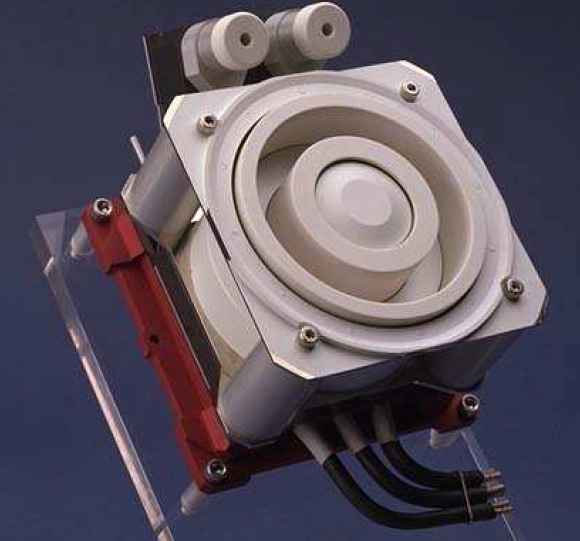
\includegraphics[width=.5\textwidth]{esempio} 
\caption{Figura mobile.\label{fig25}}
\end{figure}

Di seguito potete vedere un altro modo per inserire le unità di misura: \si{\joule\per\mole\per\kelvin}, \SI{100}{\celsius}. Oppure potete scriverle anche nel modo seguente: 78\,km/h. Per le formule chimiche potete utilizzare questa sintassi:
\ce{SO4^2- + Ba^2+ -> BaSO4 v}

La seguente è una definizione fatta per casi:
\[
n!=
\begin{cases}
1, & \text{se $n=0$,} \\
n(n-1)!, & \text{se $n\ge 1$.}
\end{cases}
\]

\chapter{Il listato del pacchetto \texttt{topcoman.sty}}
\listing{topcoman.sty}

\appendix
\chapter{Il protocollo CAN}


\begin{thebibliography}{9}
\bibitem{gal} G.~Galilei, {\em Nuovi studii sugli astri medicei}, Manuzio,
        Venetia, 1612.
\bibitem{tor1} E.~Torricelli, in ``La pressione barometrica'', {\em Strumenti
        Moderni}, Il Porcellino, Firenze, 1606.
\bibitem{tor2} E.~Torricelli e A.~Vasari, in ``Delle misure'', {\em Atti Nuovo
        Cimento}, vol.~III, n.~2 (feb. 1607), p.~27--31.
\bibitem{duane1964} Duane J.T., \emph{Learning Curve Approach To Reliability 
		Monitoring}, IEEE Transactions on Aerospace, Vol. 2, pp. 563-566, 1964
\end{thebibliography}




\end{document}

% altri riferimenti da usare come esempi.

\bibitem{chiesa2008} Chiesa S., \emph{Affidabilità, sicurezza e manutenzione 
		nel progetto dei sistemi}, CLUT, gennaio 2008
\bibitem{chiesa2}Chiesa S., Fioriti M., Fusaro R., \emph{On Board System 
		Technological  Level Improvement Effect on UAV MALE}
\bibitem{bigliano2010} Bigliano M., \emph{Sicurezza nell'installazione di un velivolo 
		senza pilota MALE; applicazione di metodologia di Zonal Safety 
		Analysis al velivolo del Progetto SAvE}, Politecnico di Torino, 
		maggio 2010
\bibitem{astrid2012} Chiesa S., Di Meo G.A., Fioriti M., Medici G., Viola N.,
		\emph{ASTRID - Aircraft on board Systems sizing and TRade-off 
		analysis in Initial Design}, Research Bulletin, Warsaw University 
		of Technology, Institute of Aeronautics and Applied Mechanics, 
		p. 1-28, 17-19, ottobre 2012

